\chapter{Estimation de la Pertinence des Descripteurs (FRE)}
\label{chap:fre}

\section{Introduction et Mission du Groupe 13}

Au sein de l'architecture de Perceptra, le module \textbf{Feature Relevance Estimation (FRE)} constitue la contribution scientifique et algorithmique assignée de manière exclusive au \textbf{Groupe 13}.

Les systèmes CBIR classiques considèrent invariablement que tous les descripteurs visuels possèdent un pouvoir discriminant équivalent. Or, l'intention de l'utilisateur est fondamentalement contextuelle~: lors de la recherche de couchers de soleil, la teinte globale et la saturation sont déterminantes, tandis que pour des textures régulières (tissus, façades), le GLCM et le LBP sont prépondérants.

L'algorithme \textbf{FRE} formalise mathématiquement cette intuition~: il observe les images annotées par l'utilisateur (pertinentes ou rejetées), quantifie la pertinence relative de chaque descripteur à partir de sa variance et de son pouvoir séparateur, et reconfigure automatiquement l'espace métrique pour les itérations suivantes.

\begin{figure}[H]
\centering
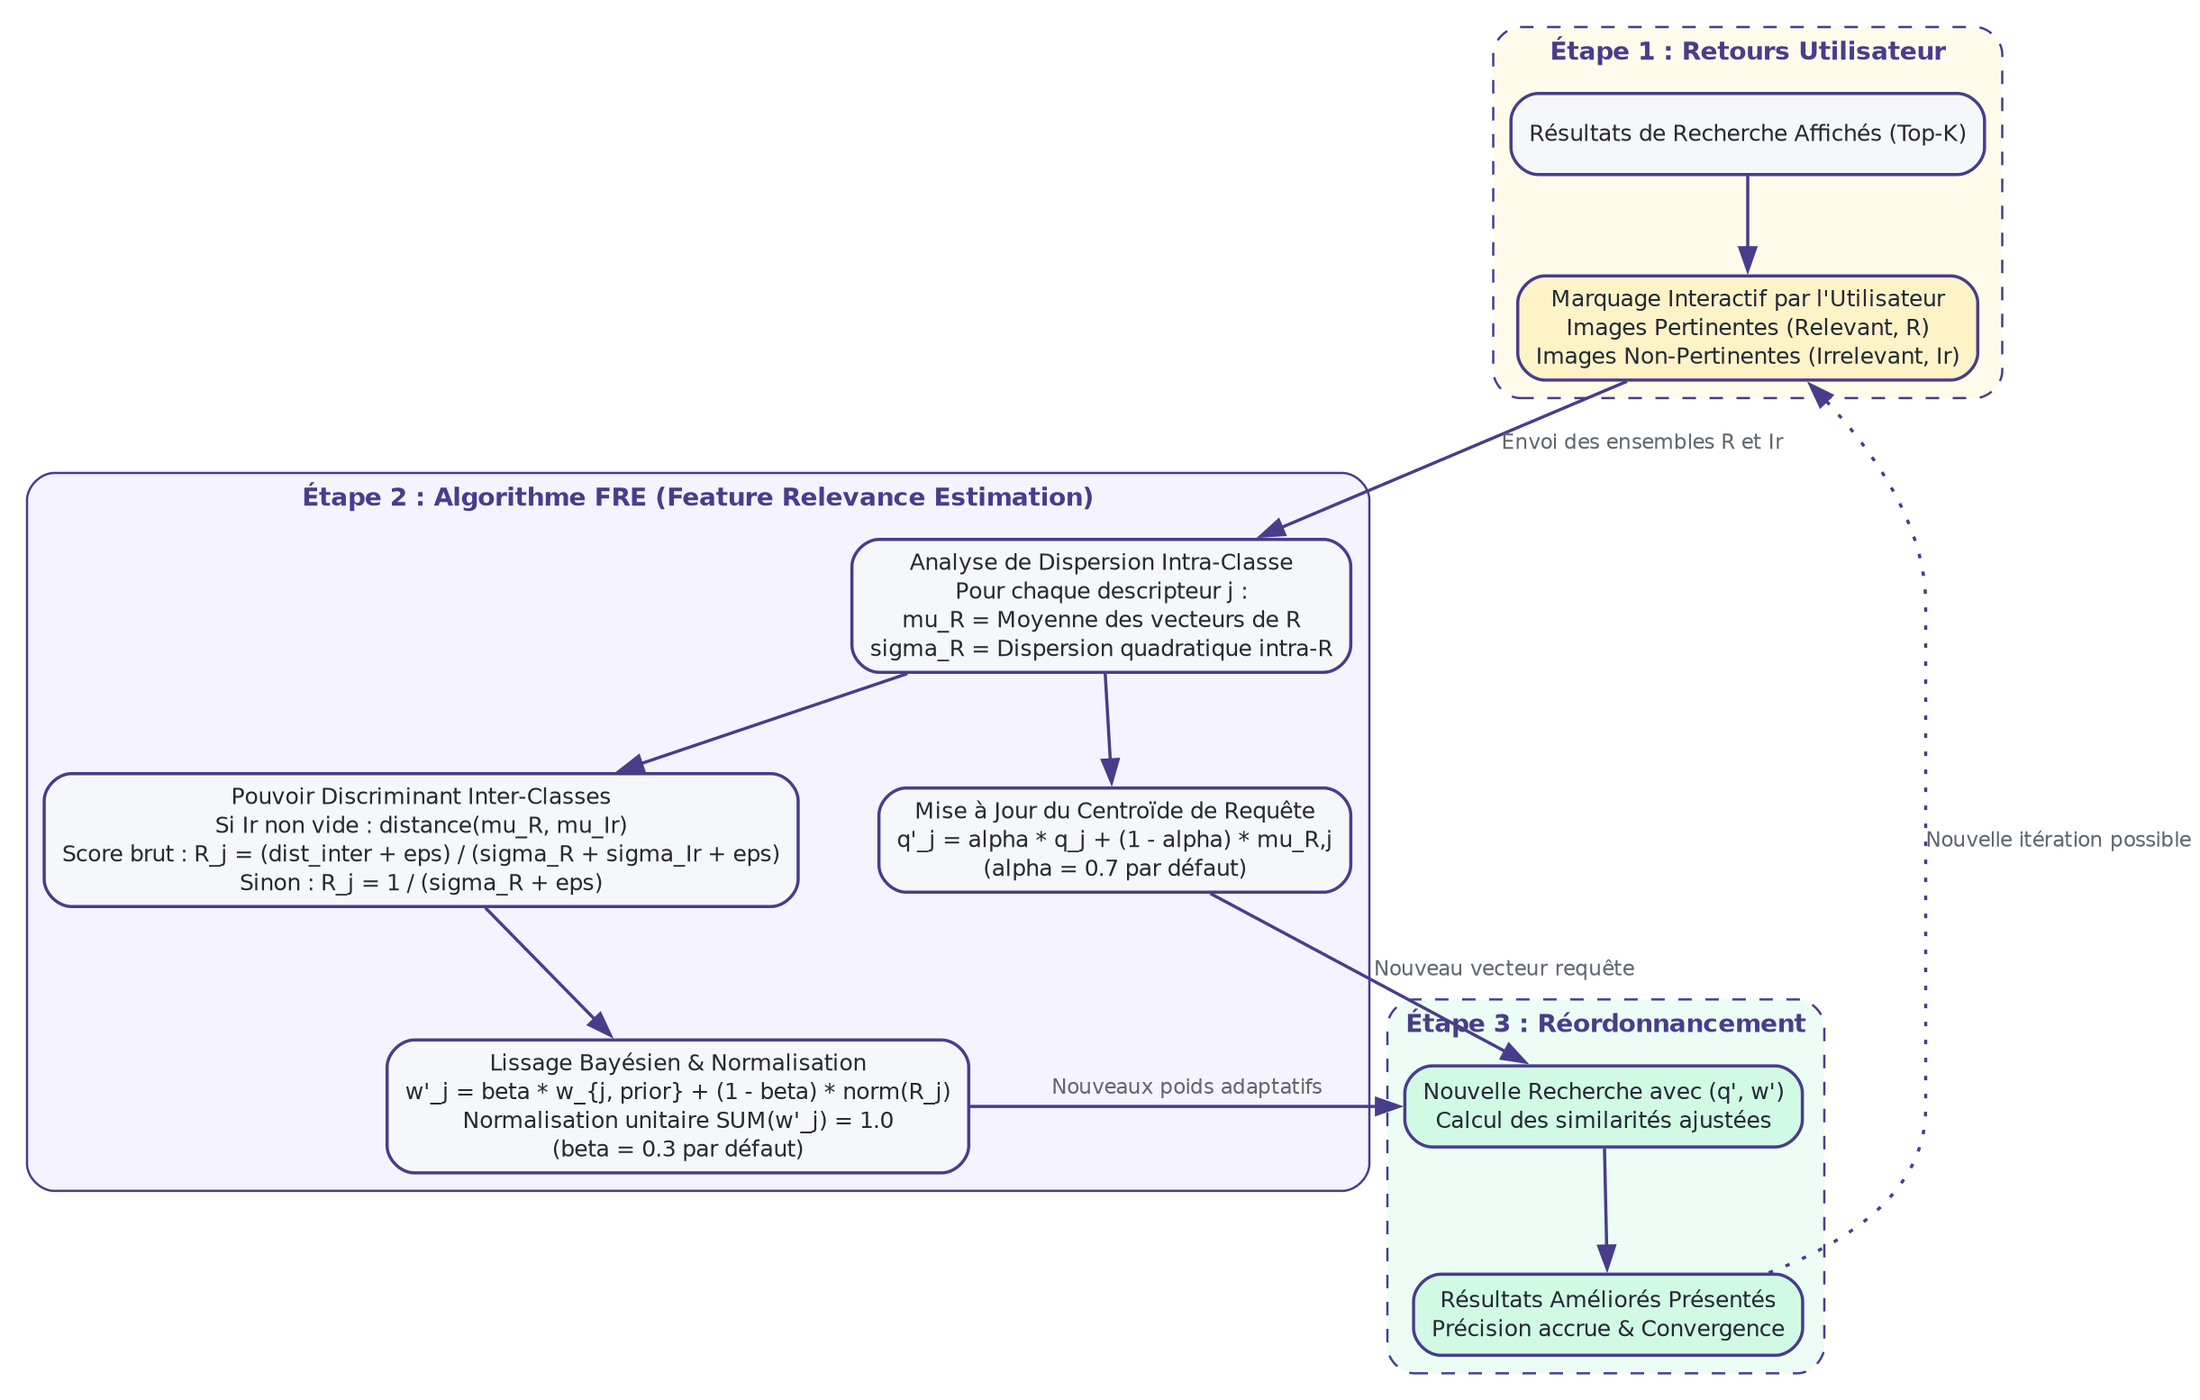
\includegraphics[width=0.66\textwidth]{images/07-boucle-relevance-feedback-fre.png}
\caption{Boucle de rétroaction adaptative FRE (Feature Relevance Estimation)}
\label{fig:boucle_fre}
\end{figure}

\section{Formulation Mathématique de l'Algorithme FRE}

Soit un espace de recherche caractérisé par un ensemble de familles de descripteurs $\mathcal{F}$. L'utilisateur labellise les résultats affichés en deux ensembles disjoints~:
\begin{itemize}
    \item L'ensemble des images pertinentes~: $\mathcal{R} = \{\mathbf{x}_1^{(r)}, \dots, \mathbf{x}_{N_r}^{(r)}\}$, avec $N_r \ge 1$~;
    \item L'ensemble des images non-pertinentes~: $\mathcal{I} = \{\mathbf{x}_1^{(i)}, \dots, \mathbf{x}_{N_i}^{(i)}\}$, avec $N_i \ge 0$.
\end{itemize}

L'algorithme se déroule en quatre étapes canoniques~:

\subsection{Étape 1 : Centroïde et Dispersion Intra-Classe}
Le centroïde de pertinence $\boldsymbol{\mu}_{R, j}$ est la moyenne arithmétique des vecteurs d'exemples positifs pour le descripteur $j$~:
\begin{equation}
\boldsymbol{\mu}_{R, j} = \frac{1}{N_r} \sum_{k=1}^{N_r} \mathbf{x}_{k, j}^{(r)}
\end{equation}

La compacité intra-classe $\sigma_{R, j}$ mesure la cohérence des exemples pertinents pour le descripteur $j$~:
\begin{equation}
\sigma_{R, j} = \begin{cases}
\sqrt{ \frac{1}{N_r} \sum_{k=1}^{N_r} \|\mathbf{x}_{k, j}^{(r)} - \boldsymbol{\mu}_{R, j}\|_2^2 } & \text{si } N_r > 1 \\
\|\mathbf{x}_{1, j}^{(r)} - \mathbf{q}_j\|_2 & \text{si } N_r = 1
\end{cases}
\end{equation}
Une faible valeur de $\sigma_{R, j}$ démontre que les exemples positifs partagent une signature quasi-identique pour le descripteur $j$, signalant une caractéristique invariante essentielle.

\subsection{Étape 2 : Séparabilité Inter-Classes (Critère de Fisher)}
Si des exemples négatifs sont fournis ($N_i \ge 1$), nous calculons leur centroïde $\boldsymbol{\mu}_{I, j}$ et leur dispersion $\sigma_{I, j}$. La distance inter-classes s'exprime par $d_{\text{inter}, j} = \|\boldsymbol{\mu}_{R, j} - \boldsymbol{\mu}_{I, j}\|_2$.

Le score brut de pertinence $R_j$ s'inspire du discriminant linéaire de Fisher (ratio entre dispersion inter et intra-classe)~:
\begin{equation}
R_j = \begin{cases}
\frac{d_{\text{inter}, j} + \epsilon}{\sigma_{R, j} + \sigma_{I, j} + \epsilon} & \text{si } N_i \ge 1 \\
\frac{1}{\sigma_{R, j} + \epsilon} & \text{si } N_i = 0
\end{cases}
\end{equation}
où $\epsilon = 10^{-4}$ prévient toute division par zéro.

\subsection{Étape 3 : Lissage Bayésien et Normalisation des Poids}
Les scores bruts sont normalisés sous contrainte unitaire $\tilde{R}_j = R_j / \sum_{k \in \mathcal{F}} R_k$. Afin d'éviter les sur-ajustements (\textit{overfitting}) lors des premiers retours, un paramètre de lissage avec mémoire d'inertie $\beta \in [0, 1]$ (fixé à $\beta = 0.3$) combine les poids a priori avec la nouvelle estimation~:
\begin{equation}
w'_j = \beta \cdot w_{j, \text{prior}} + (1 - \beta) \cdot \tilde{R}_j \implies w_{j, \text{final}} = \frac{w'_j}{\sum_{k \in \mathcal{F}} w'_k}
\end{equation}

\subsection{Étape 4 : Déplacement Guidé du Centroïde de Requête}
Parallèlement à l'ajustement des poids, le vecteur de requête $\mathbf{q}_j$ est translaté vers le barycentre des exemples positifs via un coefficient de momentum $\alpha = 0.7$~:
\begin{equation}
\mathbf{q}'_j = \alpha \cdot \mathbf{q}_j + (1 - \alpha) \cdot \boldsymbol{\mu}_{R, j}
\end{equation}

\section{Implémentation Logicielle et Diagnostics}

L'implémentation de ce modèle dans la classe \texttt{FeatureRelevanceEstimator} (\texttt{src/services/relevance\_feedback.py}) garantit une convergence rapide et une stabilité numérique totale.

\begin{lstlisting}[language=Python, caption={Extrait central de l'algorithme FRE (src/services/relevance\_feedback.py)}]
# Critere de type Fisher : ecart inter-classe / dispersion intra-classe
if irr_vecs:
    irr_mat = np.vstack(irr_vecs)
    mu_irr = np.mean(irr_mat, axis=0)
    between_distance = float(np.linalg.norm(mu_r - mu_irr))
    dispersion_irr = np.sqrt(max(0.0, float(np.mean(np.sum((irr_mat - mu_irr)**2, axis=1)))))
    relevance_val = (between_distance + cls.EPSILON) / (dispersion_r + dispersion_irr + cls.EPSILON)
else:
    between_distance = 0.0
    relevance_val = 1.0 / (dispersion_r + cls.EPSILON)

# Deplacement du centroide de requete
refined_q = alpha_query * q_vec + (1.0 - alpha_query) * mu_r

# Lissage avec la configuration a priori
blended = beta_prior * prior_w + (1.0 - beta_prior) * norm_estimated[ft]
\end{lstlisting}
